\documentclass[10pt, xcolor=x11names,compress, aspectratio=169]{beamer}
\usepackage{tabulary}
\usepackage{booktabs}
\usepackage{float}
\usepackage{graphicx}
\graphicspath{{../Figures/}}
\usepackage{mwe}% for example pictures
\usepackage{siunitx}
\usepackage{hyperref}

\usecolortheme{dolphin}

% set colors
\definecolor{myNewColorA}{RGB}{25,25,112}
\definecolor{myNewColorB}{RGB}{25,25,112}
\definecolor{myNewColorC}{RGB}{25,25,112}
\setbeamercolor*{palette primary}{bg=myNewColorC}
\setbeamercolor*{palette secondary}{bg=myNewColorB, fg = white}
\setbeamercolor*{palette tertiary}{bg=myNewColorA, fg = white}
\setbeamercolor*{titlelike}{fg=myNewColorA}
\setbeamercolor*{title}{bg=myNewColorA, fg = white}
\setbeamercolor*{item}{fg=myNewColorA}
\setbeamercolor*{caption name}{fg=myNewColorA}
\usefonttheme{professionalfonts}
\useoutertheme{infolines}
\setbeamertemplate{headline}[default]
\setbeamertemplate{navigation symbols}{}
\mode<beamer>{\setbeamertemplate{blocks}[rounded][shadow=true]}
\setbeamercovered{transparent}
\makeatletter\setbeamertemplate{footline}
{  
\leavevmode%  
\hbox{%  
\begin{beamercolorbox}[wd=.333333\paperwidth,ht=2.25ex,dp=1ex,center]{author in head/foot}%    
\usebeamerfont{author in head/foot}
\insertshortauthor%~~\beamer@ifempty{\insertshortinstitute}{}
 \end{beamercolorbox}%  
 \begin{beamercolorbox}[wd=.333333\paperwidth,ht=2.25ex,dp=1ex,center]{institute in head/foot}%    
 \usebeamerfont{title in head/foot}\insertinstitute  
 \end{beamercolorbox}%  
 \begin{beamercolorbox}[wd=.333333\paperwidth,ht=2.25ex,dp=1ex,right]{date in head/foot}%    
 \usebeamerfont{date in head/foot}\insertshortdate{}\hspace*{2em}    
 \insertframenumber{} / \inserttotalframenumber\hspace*{2ex}   
 \end{beamercolorbox}}%  
 \vskip0pt%
 }
 \makeatother 
 \useoutertheme[footline=empty, subsection=false]{miniframes}
 \usepackage{multicol}  
 \author{Presented by Emily WANG}
 \title{Deviation from a Good Will: Land Misallocation under Imperfect Monitoring in China}
 \subtitle{Research Proposal}

 \institute{University of Tokyo}\date{10/2025} 
 \begin{document}
 \begin{frame}
 \titlepage
 \end{frame}

\section*{Introduction}

\begin{frame}{Motivation}

\begin{itemize}
    \item In a centralized system, the \textbf{central government} delegates development and policy targets to \textbf{lower-level governments}.
    \begin{itemize}
        \item Local officials have \textbf{promotion incentives} to meet these targets under a performance-based evaluation system.
        \item However, the target-based system functions as an \textbf{imperfect monitoring mechanism}.
        \item $\Rightarrow$ This may induce a phenomenon of \textbf{``form over function''}: meeting the appearance of compliance rather than the substance of performance.
    \end{itemize}

    \vspace{1em}
    \item \textbf{Research Questions:}
    \begin{enumerate}
        \item Does ``form over function'' arise when monitoring is imperfect?
        \item Who bears the cost of such distortions under imperfect monitoring?
        \begin{itemize}
            \item TBD
        \end{itemize}
    \end{enumerate}
\end{itemize}

\end{frame}



\begin{frame}{Timeline}
\begin{figure}[H]
    \centering
    
\includegraphics[width=1\textwidth]{timeline.png}
\end{figure}
\end{frame}


\begin{frame}{Motivation: Land Policy in China}
\begin{itemize}
    \item \textbf{"Red Line" Policy in China}: 
\begin{itemize}
    \item China's total arable land shall be no less than 1.8 billion \emph{mu} (120 million hectares)
    \item 2005: The State Council released assessment measures for provincial governments\footnote{\footnotesize \href{https://www.gov.cn/gongbao/content/2005/content_129504.htm}{Document of 2005 policy}}
    \item \textcolor{blue}{2018}: A revised version has been introduced to assess local land protection more \textcolor{blue}{stringently}\footnote{ \href{https://www.gov.cn/zhengce/content/2018-01/18/content_5257943.htm}{Document of 2018 policy}}
\end{itemize}
\end{itemize}

\begin{figure}[H]
    \centering
    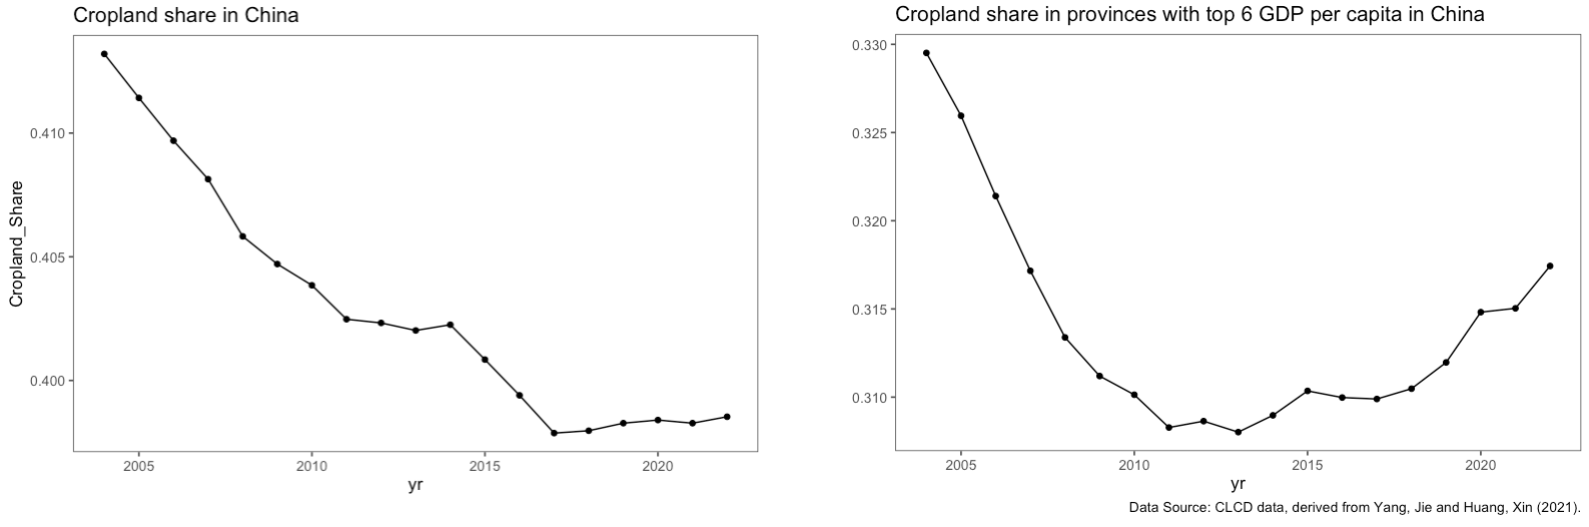
\includegraphics[width=0.8\textwidth]{cropshare_combined.png}
\end{figure}

\end{frame}

\begin{frame}{Motivation: Land Policy in China}
\begin{figure}[H]
    \centering
    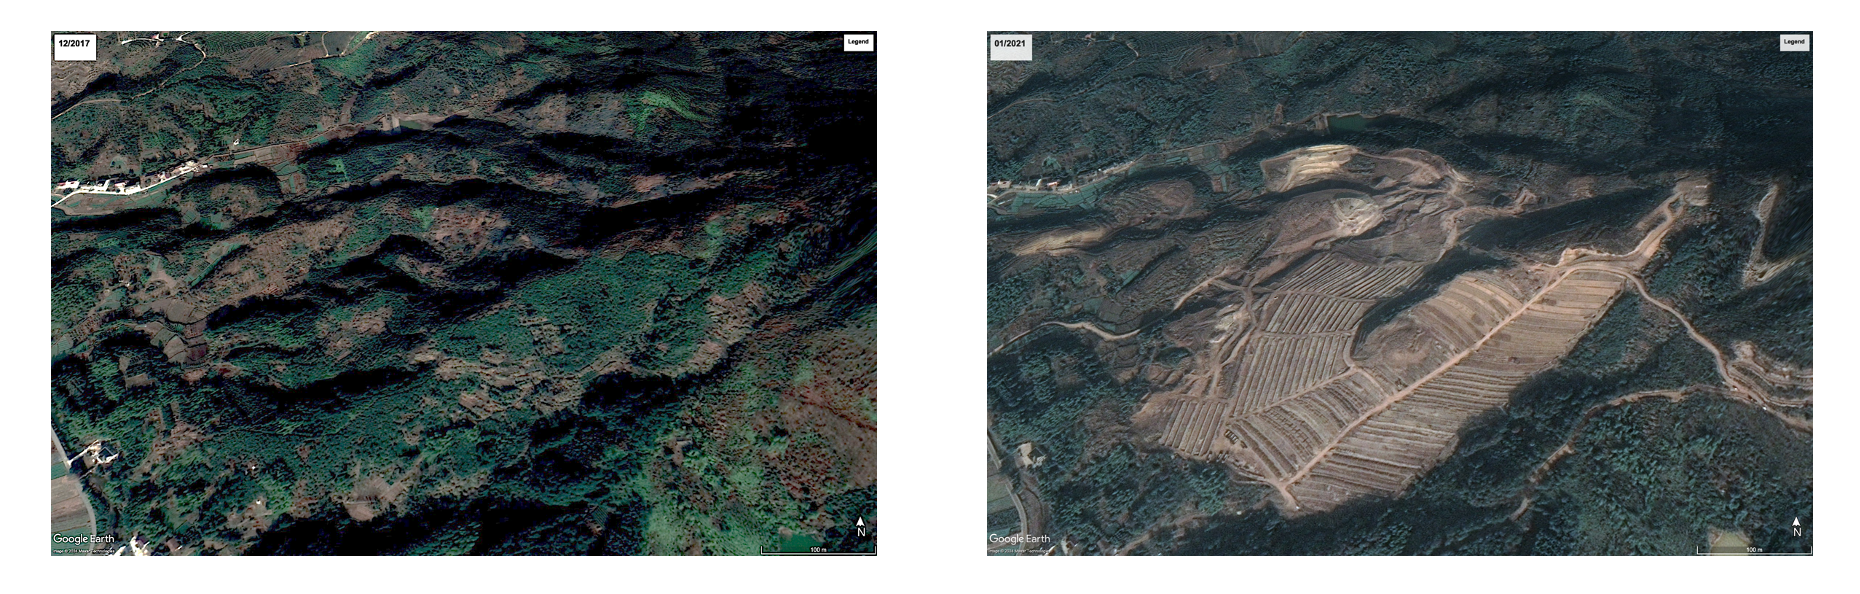
\includegraphics[width=0.8\textwidth]{anecdote_both.png}
    \caption{An example of local policy implementation: forest $\rightarrow$ terrace}
\end{figure}
\begin{itemize}
    \item \textbf{Anecdotes on deviation in local enforcement}: 
    \begin{itemize}
        \item Green for grain, Rice on mountain
        \item \textcolor{blue}{Allocative inefficiency}
    \end{itemize}
\end{itemize}
\end{frame}

\begin{frame}{Motivation: Land Policy in China}

\begin{itemize}
    \item China’s central government enforces a strict \textbf{cropland protection policy} (the ``red-line'' policy) to ensure national food security.
    \begin{itemize}
        \item Each administrative level---province, city, and county---is assigned cropland preservation targets that must be met or exceeded.
        \item These targets emphasize maintaining the \textbf{total area} of cultivated land rather than its actual use or productivity.
    \end{itemize}

    \vspace{1em}

    \item The monitoring system is \textbf{imperfect}.
    \begin{itemize}
        \item Higher-level governments can easily verify \textbf{land area} through remote sensing and administrative reports.
        \item However, they face substantial difficulty in observing the \textbf{actual cultivation or quality of use} on the ground.
        \item $\Rightarrow$ This asymmetric observability creates incentives for local officials to reclaim marginal or unsuitable land simply to satisfy quantitative area targets.
    \end{itemize}

    \vspace{1em}

    \item As a result, cropland statistics may reflect \textbf{``form over function''}---compliance in appearance, but with limited productive use.
\end{itemize}

\end{frame}

\begin{frame}{Research Overview}
\hypertarget{overview}{}
\begin{itemize}
    \item \textbf{Research Question (RQ):} Under a target-based performance evaluation system that explicitly counts cropland size (introduced in 2018), do local officials in land-scarce regions exhibit a higher incidence of inefficient cropland expansion?
    \vspace{0.5em}
    \item \textbf{Hypothesis 1 (Extensive Margin):} 
    Prefectures with tighter land constraints respond more strongly to the cropland protection assessment, leading to a larger post-2018 increase in cropland share.
    \begin{itemize}
        \item \textbf{Outcome:} Cropland share (grid level)
        \item \textbf{Treatment intensity:} Although the 2018 cropland protection policy was implemented nationwide, its \textbf{binding intensity} varies across prefectures depending on pre-existing \textbf{land scarcity}.
        \item \hyperlink{balancepolicy}{\beamergotobutton{Policy details}} \quad \hyperlink{preliminaryresult}{\beamergotobutton{Preliminary results}}
    \end{itemize}
\end{itemize}
\end{frame}

\begin{frame}{Research Overview (cont.)}
\begin{itemize}
    \item \textbf{Hypothesis 2 (Intensive Margin / Efficiency):}
    Following the 2018 policy, in prefectures where land resources are scarce and provincial leaders face stronger incentives to fulfill cropland targets, newly reclaimed land is more likely to be abandoned shortly after reclamation.
    \vspace{0.5em}
    \begin{itemize}
        \item \textbf{Proxy for land scarcity:} Share of non-urban (available) land in total prefectural area
        \item \textbf{Proxy for land abandonment:} Fractional Vegetation Cover (FVC) and Normalized Difference Vegetation Index (NDVI)
    \end{itemize}
\end{itemize}
\end{frame}



\begin{frame}{Contribution to literature}
\begin{itemize}
    \item \textbf{Land regulation}: 
    \begin{itemize}
    \item housing prices (Hilber and Vermeulen, 2016), economic growth (Besley and Burgess, 2000), farmer-level productivity (Beg, 2022; Adamopoulos et al., 2022 (resource misallocation across farmer; my study: misallocation across land))
    \item Chinese context: Henderson et al. (2022), Cai et al. (2017), Adamopoulos (2022), Cheng and Chung (2018)
    \end{itemize}
    \item \textbf{Political economy in a centralized regime}: 
    \begin{itemize}
        \item Theory: principal-agent problem (Ross, (1973)), overcentralization (Kornai, (1959)), multi-tasking (Holmstrom and Milgrom (1991), Hart, Shleifer, and Vishny (1997))  
        \item Empirical studies: environmental regulation (Fan et al., (2023), Chen et al., (2018), He et al., (2020))
    \end{itemize}
    \item \textbf{Contribution}: 
    \begin{itemize}
        \item \textcolor{blue}{Cropland protection regulation-induced cropland misallocation: Extensive Margin $\checkmark$, Intensive Margin X}
        \item \textcolor{blue}{Exacerbate regional inequality}
    \end{itemize}
\end{itemize}
\end{frame}

\begin{frame}{Data}
\begin{itemize}
    \item Cropland data:
    \begin{itemize}
        \item Raster data: The 30 m annual land cover dataset and its dynamics in China from 1990 to 2022 (\textcolor{blue}{now using 2011 - 2022})
        \item County-level data: Statistical yearbook of China
    \end{itemize}
    \item 2010 census data: \textcolor{blue}{info on urban density, population, GDP...}
    \item Soil property data: cross-section
    \item Topographical data: cross-section
    \item Bureaucrats data: prefecture-, and province-level officials (gender, age, education, ethnicity, hometown, and tenure) from 1992 - 2022
    \item Old administrative division (Qing dynasty), location of historical villages
\end{itemize}
\end{frame}

\section*{Theoretical Model}
\begin{frame}{Principal-Agent Model with Imperfect Information/ Moral Hazard Model}
    TBD
\end{frame}


\section*{Extensive Margin}

\begin{frame}{Preliminary analysis on cropland share}
\hypertarget{preliminaryresult}{}
\begin{itemize}
    \item A small-scale analysis in one province - Jiangsu province: (1) top-ranked GDP per capita, (2) covered by plain
\begin{figure}[H]
    \centering
    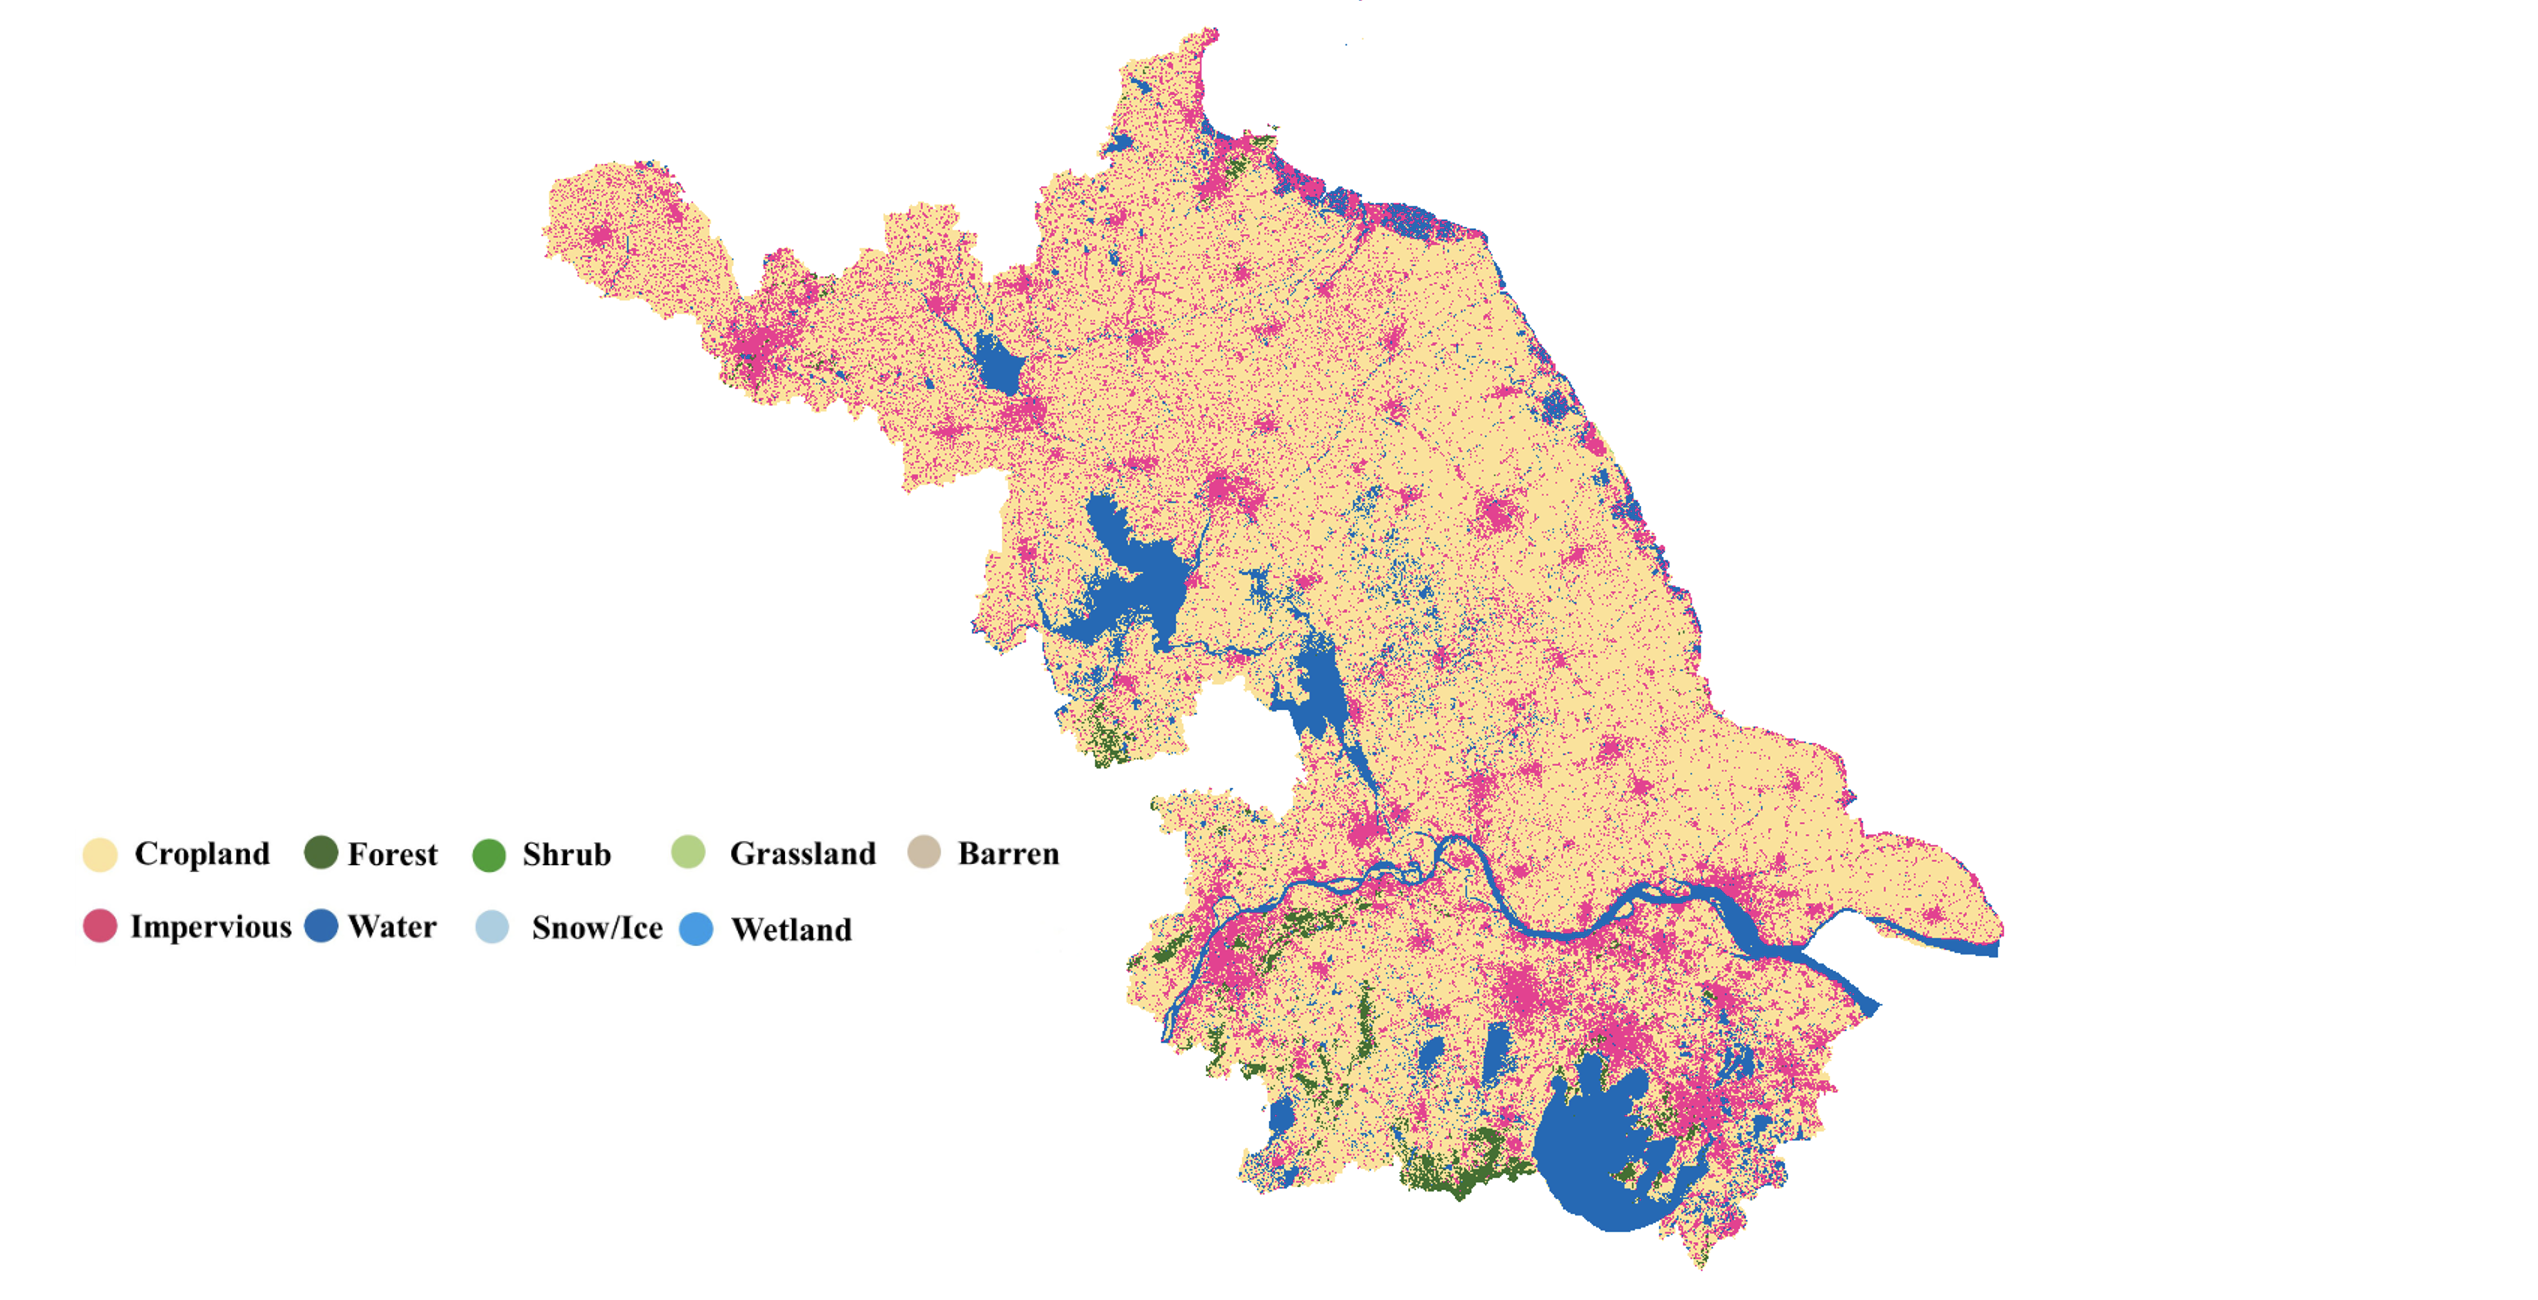
\includegraphics[width=0.8\textwidth]{jiangsu.png}
\end{figure}
\end{itemize}
\end{frame}

\begin{frame}{Preliminary analysis on cropland share}
\hypertarget{preliminaryresult}{}
\begin{itemize}
\begin{figure}[H]
    \centering
    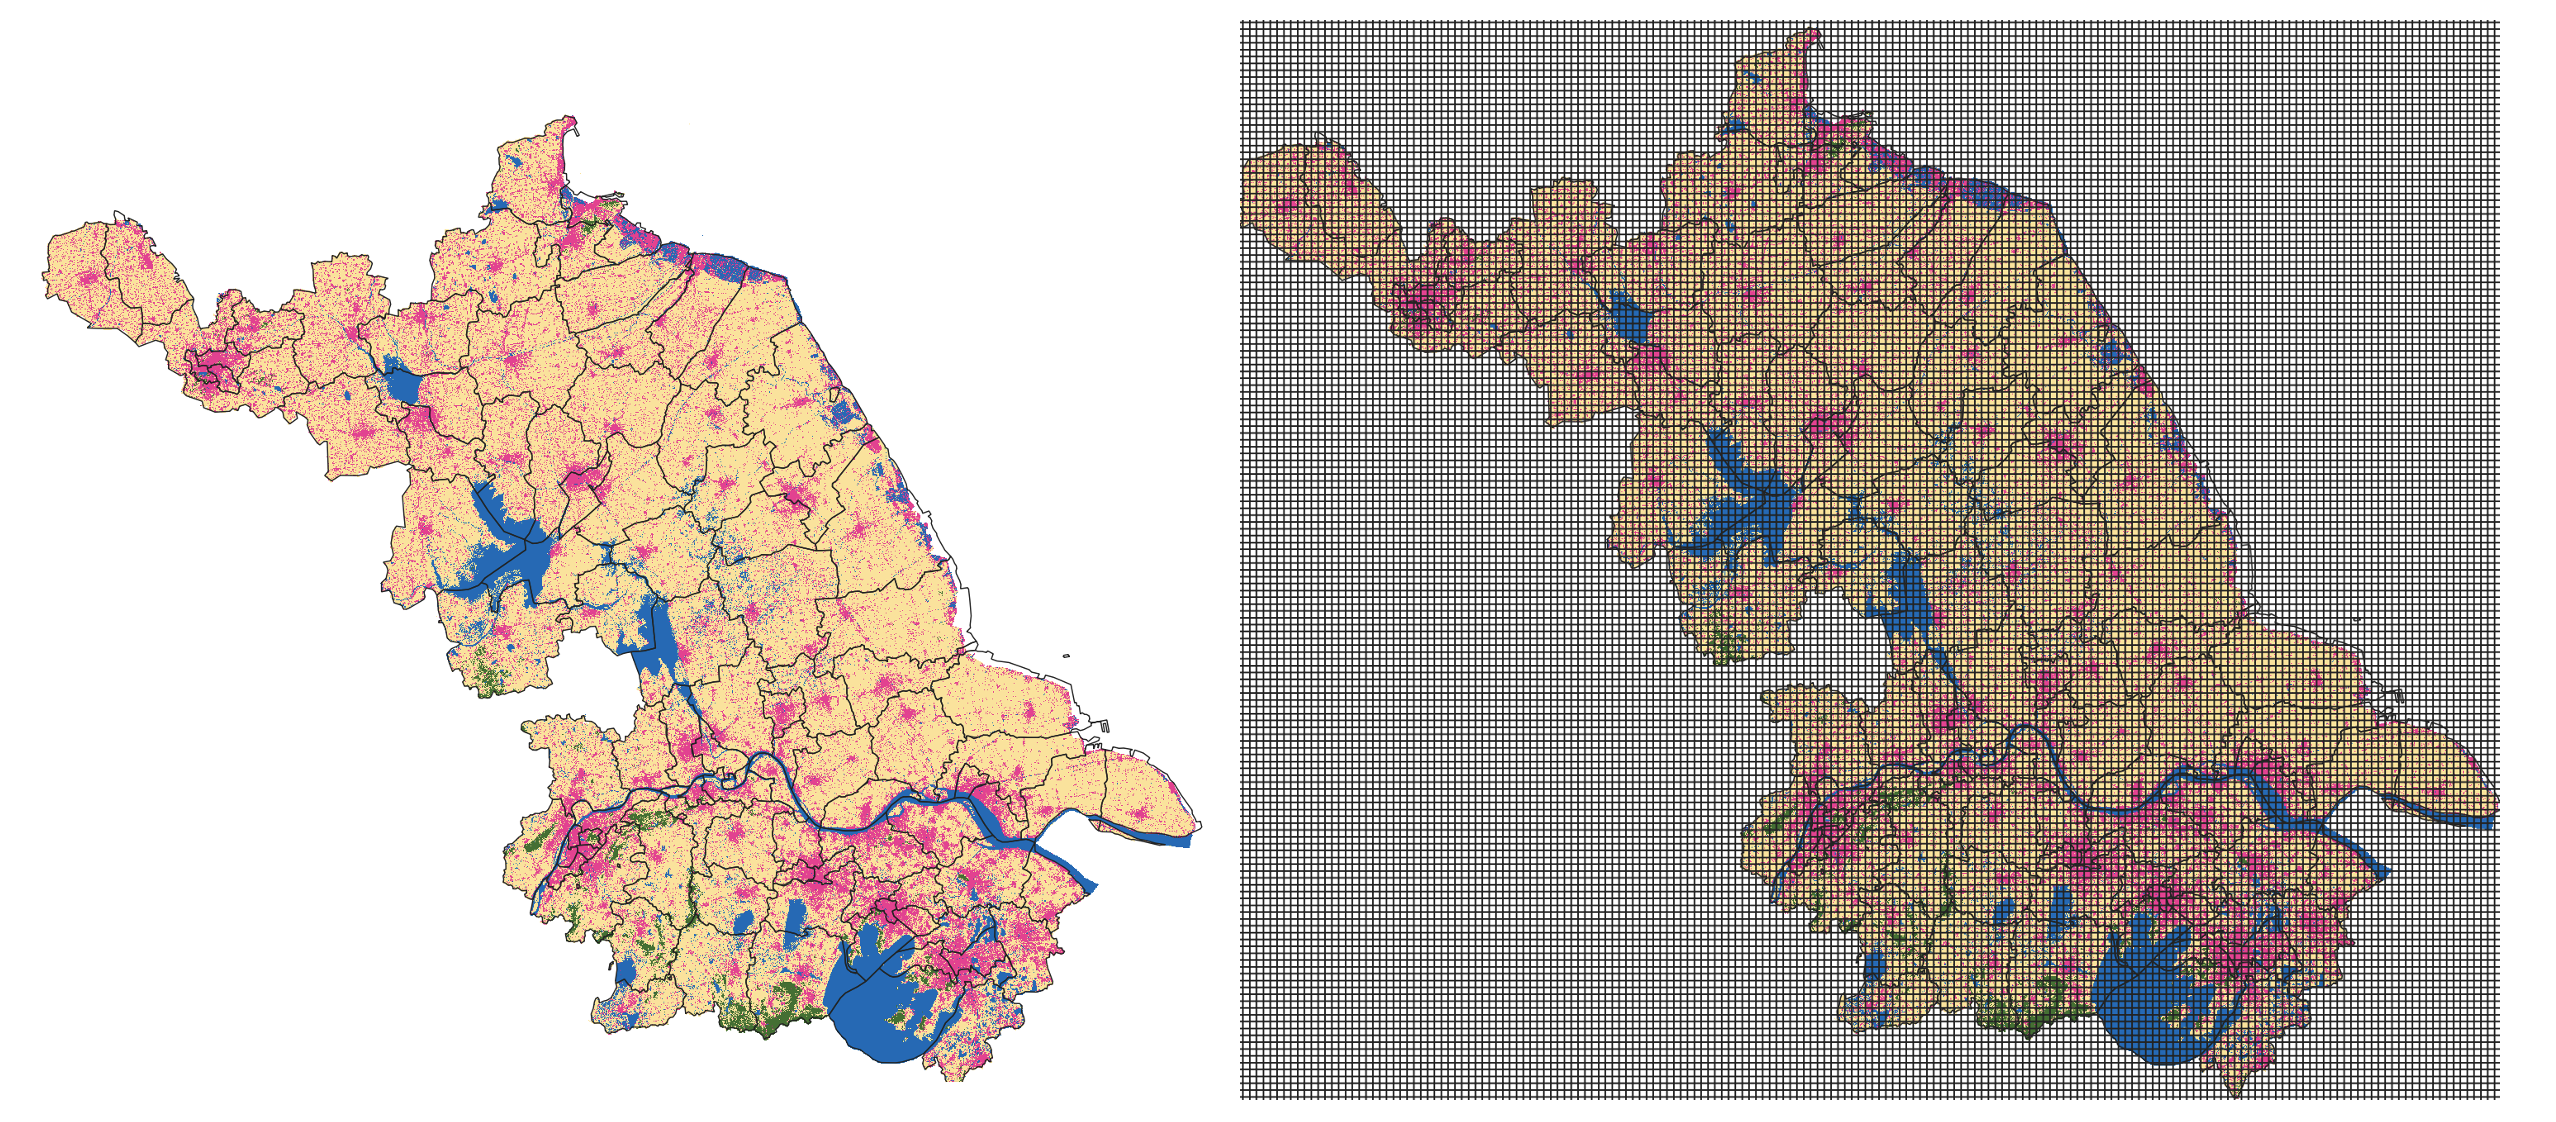
\includegraphics[width=0.8\textwidth]{jiangsu_procedure.png}
\end{figure}
\end{itemize}
\end{frame}

\begin{frame}{Identification and Empirical Specification}

\begin{itemize}
    \item The 2018 cropland protection policy was implemented nationwide, 
    but its \textbf{binding intensity} varies across prefectures.
    \begin{itemize}
        \item Prefectures with \textbf{scarce land resources} faced tighter 
        cropland quotas and stronger incentives to expand reported cropland area.
        \item Prefectures with \textbf{abundant land} experienced weaker policy pressure.
    \end{itemize}

    \vspace{1em}

    \item \textbf{Identification assumption:}
\begin{itemize}
    \item The \textit{urban share} (the share of urban administrative divisions within a prefecture)
    captures the \textbf{pre-determined land scarcity} that governs the binding strength of the 2018 policy.
    \item Conditional on fixed effects, \textit{urban share} is statistically independent of 
    contemporaneous shocks to cropland expansion, providing quasi-exogenous variation 
    in policy intensity across prefectures.
\end{itemize}

    \vspace{1em}

\begin{block}{Empirical specification (TWFE):}
\[
    \text{crop\_share}_{it} = 
    \sum_{k \neq 0} 
    \beta_k \big(\text{UrbanShare}_{p(i)} \times \text{Event}_{k,t}\big)
    + \mu_i + \lambda_t + \varepsilon_{it}
\]
\end{block}
\end{itemize}

\end{frame}




\begin{frame}{Eevent study plot}

\begin{figure}[H]
    \centering
    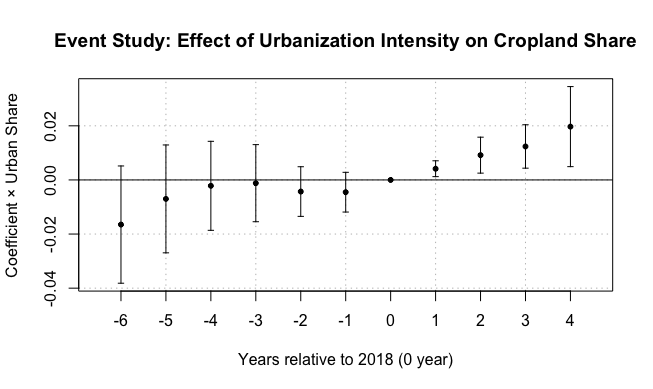
\includegraphics[width=0.7\textwidth]{extensive_eventstudy.png}
\hyperlink{overview}{\beamerreturnbutton{Return}}
\end{figure}
\end{frame}

\section*{Intensive Margin}

\begin{frame}{Data and Key Definitions}
\begin{itemize}
    \item \textbf{Observation unit:} 500 $\times$ 500 \textbf{grid cell}

    \vspace{0.8em}
    \item \textbf{Cropland data (CLCD, 2011–2022):}
    \begin{itemize}
        \item 30m annual land cover classification for China (resampled to Albers projection)
        \item Identifies \emph{newly cultivated pixels} each year (first transition into cropland)
        \item Grid-level \textbf{cropland share} = share of pixels classified as cropland
        \item \textbf{Definition of reclaimed cropland:} a grid is defined as \textit{newly reclaimed} in year $t$
              if its cropland share rises from below 0.6 in $t$ to above 0.7 in both $t\!+\!1$ and $t\!+\!2$.
    \end{itemize}

    \vspace{0.8em}
    \item \textbf{Vegetation data (FVC, 2010–2022):}
    \begin{itemize}
        \item 30m / 15-day Fractional Vegetation Cover (FVC) dataset 
        \item Derived from Landsat-based NDVI using a pixel-wise dimidiate model
        \item Values: 0–100 (scaling factor 0.01), higher $\Rightarrow$ denser vegetation
    \end{itemize}

    \vspace{0.8em}
    \item \textbf{Definition of land abandonment:}
    \begin{itemize}
        \item For each newly reclaimed grid $i$ (first cultivated in $t_0$), 
              measure whether annual average FVC in $t_0\!+\!1$ or $t_0\!+\!2$ falls below a threshold (e.g., 0.3)
        \item Grid-level \textbf{fallow rate} = share of reclaimed pixels with low FVC
    \end{itemize}
\end{itemize}
\end{frame}



\begin{frame}{Empirical Strategy: Intensive Margin}
\begin{itemize}
    \item \textbf{Objective:} Examine whether newly reclaimed land is more likely to be \textbf{abandoned} in prefectures facing tighter land constraints after the 2018 cropland assessment reform.
    \vspace{0.5em}
    \item \textbf{Observation unit:} Newly reclaimed pixel or land patch $i$ within grid $c(i)$
    \begin{itemize}
        \item Cohort (reclamation year): $t_0(i) \in \{2014, \ldots, 2021\}$
        \item Post-reclamation years: $s \in \{1,2\}$
        \item Outcome: $Y_{i,s}=1$ if pixel $i$ is abandoned in $t_0(i)+s$
    \end{itemize}
    \vspace{0.5em}
    \item \textbf{Treatment intensity:}
    \[
        W_i = 1\{t_0(i)>2018\} \times Z_{c(i)}
    \]
    where $Z_{c(i)}$ measures prefectural land scarcity (Higher urban share $\Rightarrow$ higher constraint).
\end{itemize}
\end{frame}

\begin{frame}{Empirical Strategy: Continuous-Treatment Cohort DID}
\begin{itemize}
    \item \textbf{Estimation:}
    \[
        Y_{i,s} = \alpha_{c(i)} + \mu_{t_0(i)} + \delta_s 
        + \beta W_i + X_{i}'\gamma + \varepsilon_{i,s}
    \]
    \vspace{0.5em}
    \item \textbf{Interpretation:}
    \begin{itemize}
        \item $\beta$: policy effect on abandonment --- 
        within the same cohort, prefectures with higher $Z_c$ (tighter constraints) show stronger post-2018 abandonment.
        \item $\alpha_{c(i)}$: prefecture FE (absorbing spatial heterogeneity)
        \item $\mu_{t_0(i)}$: cohort FE (absorbing time of reclamation)
        \item $\delta_s$: years-since-reclamation FE (1st or 2nd year)
    \end{itemize}
    \vspace{0.5em}
    \item \textbf{Standard errors:} Cluster by prefecture, spatially adjusted (Conley).
    \item \textbf{Interpretation:} This is a \emph{Post $\times$ Intensity} design across cohorts, identifying heterogeneity in policy response rather than timing.
\hyperlink{overview}{\beamerreturnbutton{Return}}
\end{itemize}
\end{frame}

\begin{frame}{Effect of Land Policy on Fallow Rate (Cohort-DiD)}
\begin{table}[h!]
\centering
\footnotesize
\begin{tabular}{lccc}
\hline\hline
 & (1) First Year ($s=1$) & (2) Second Year ($s=2$) & (3) Pooled ($s=1,2$) \\
\hline
\textbf{Dependent variable:} & \multicolumn{3}{c}{Fallow rate of newly reclaimed land} \\
\\[-0.7em]
$W$ (Post $\times$ Urban share) & 0.472$^{***}$ & 0.010 & 0.241$^{**}$ \\
 & (0.118) & (0.097) & (0.104) \\
\\[-0.7em]
Observations & 1,172 & 1,171 & 2,343 \\
Adj. $R^2$ & 0.179 & 0.204 & 0.191 \\
Within $R^2$ & 0.013 & 0.000 & 0.004 \\
Fixed effects & Prefecture, Cohort & Prefecture, Cohort & Prefecture, Cohort \\
RMSE & 0.444 & 0.442 & 0.447 \\
\hline
\multicolumn{4}{l}{\footnotesize Clustered standard errors at the prefecture level.} \\
\multicolumn{4}{l}{\footnotesize $^{***}p<0.01$, $^{**}p<0.05$, $^{*}p<0.1$.} \\
\hline\hline
\end{tabular}
\end{table}

\begin{itemize}
    \item Fallow rate rises sharply in the first year after reclamation in land-scarce (urbanized) prefectures.  
    \item No significant effect in the second year, suggesting that most abandoned plots recover within two years.  
    \item The pooled estimate confirms a statistically significant but moderate short-term distortion.
\end{itemize}

\end{frame}


\begin{frame}{Before-After Analysis}

\begin{itemize}
    \item \textbf{Specification:}
    \[
        \text{fallow}_{ip} = \alpha + \beta W_p + \mu_p + \varepsilon_{ip}
    \]
    where $\mu_p$ are prefecture fixed effects and standard errors are clustered at the prefecture level.

    \vspace{0.8em}
    
    \item \textbf{Interpretation:}
    \begin{itemize}
        \item $W_p = 1$ if the prefecture’s newly reclaimed land cohort falls under the post-2018 policy regime.
        \item $\text{fallow}_{ip}$ indicates whether grid $i$ shows vegetation loss (FVC $<0.3$) one or two years after reclamation.
    \end{itemize}

    \vspace{0.8em}
    \item \textbf{Results:}
    \begin{table}[h!]
    \centering
    \footnotesize
    \begin{tabular}{lccc}
    \hline\hline
    & (1) $s=1$ & (2) $s=2$ & (3) Pooled \\
    \hline
    \textbf{Dependent variable:} & \multicolumn{3}{c}{Fallow rate of newly reclaimed grids} \\
    \\[-0.7em]
    $W$ (Post-2018) & 0.148$^{*}$ & 0.155$^{***}$ & 0.151$^{**}$ \\
    & (0.071) & (0.036) & (0.046) \\
    \\[-0.7em]
    Observations & 1,172 & 1,171 & 2,343 \\
    Adj. $R^2$ & 0.127 & 0.184 & 0.162 \\
    Within $R^2$ & 0.019 & 0.022 & 0.021 \\
    Fixed effects & Prefecture & Prefecture & Prefecture \\
    RMSE & 0.460 & 0.449 & 0.456 \\
    \hline
    \multicolumn{4}{l}{\footnotesize Clustered SEs at prefecture level. $^{***}p<0.01$, $^{**}p<0.05$, $^{*}p<0.1$.}\\
    \hline\hline
    \end{tabular}
    \end{table}

    \vspace{0.5em}
    \item \textbf{Implication:}  
    Post-2018 land reclamation significantly increases the likelihood of fallowing, suggesting that 
    prefectures under tighter land constraints exhibit stronger “\textit{form over function}” behavior 
    when meeting cropland targets.
\end{itemize}

\end{frame}





\section*{Appendix}

\begin{frame}{Cropland policy intensity}
\hypertarget{balancepolicy}{}
\begin{itemize}
    \item \textbf{Cropland protection policy is binding more on prefectures with}
    \begin{enumerate}
    \item Higher \textcolor{population density} in urban density: urbanization, economic growth
    \item Higher \textcolor{blue}{urban share} in prefecture
    \end{enumerate}
\end{itemize}
\indent \emph{\textbf{Cropland balance policy} "If they (local governments) are unable to independently compensate with an equivalent amount and quality of arable land, they must pay the arable land reclamation fee in full as required. Local governments at all levels are responsible for organizing and implementing land consolidation ... The primary method is \textcolor{blue}{(1) self-balancing within counties, (2) supplemented by adjustments within provinces, and (2) further supplemented by appropriate national coordination}, to fulfill the task of compensating for arable land."}
\end{frame}

\begin{frame}{Example on high urban share v.s. low urban share}
\begin{figure}
    \centering
    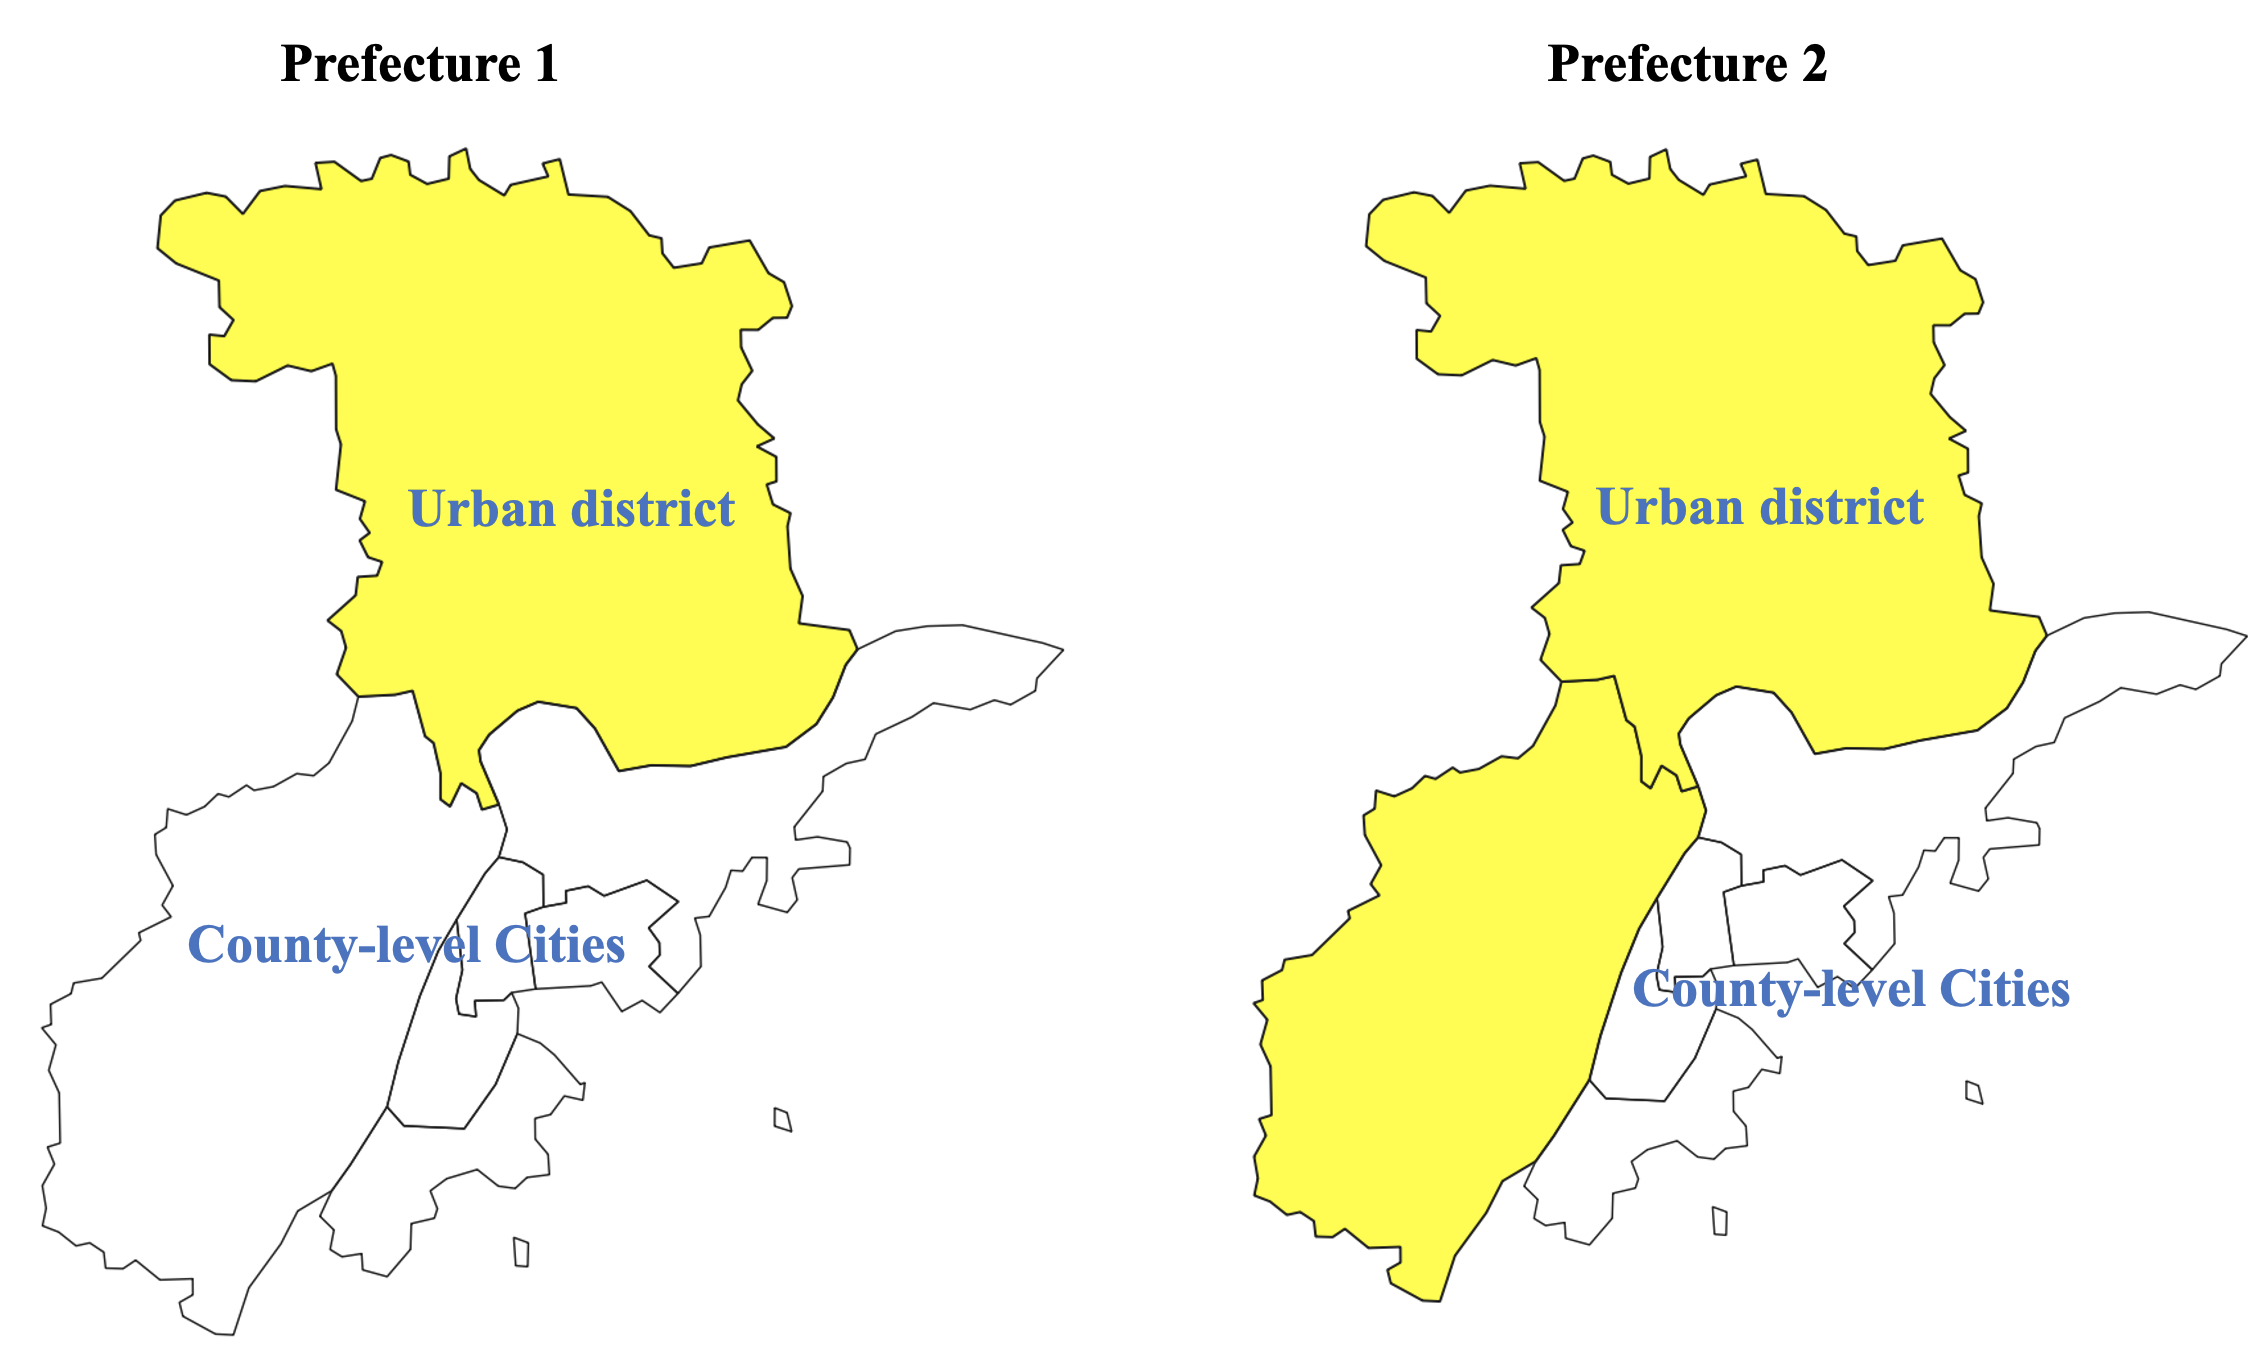
\includegraphics[width=0.8\textwidth]{example.png}
\end{figure}
\hyperlink{overview}{\beamerreturnbutton{Return}}
\end{frame}



\end{document}

\begin{frame}{Descriptive statistics: high urban share v.s. low urban share}
\begin{figure}[H]
    \centering
    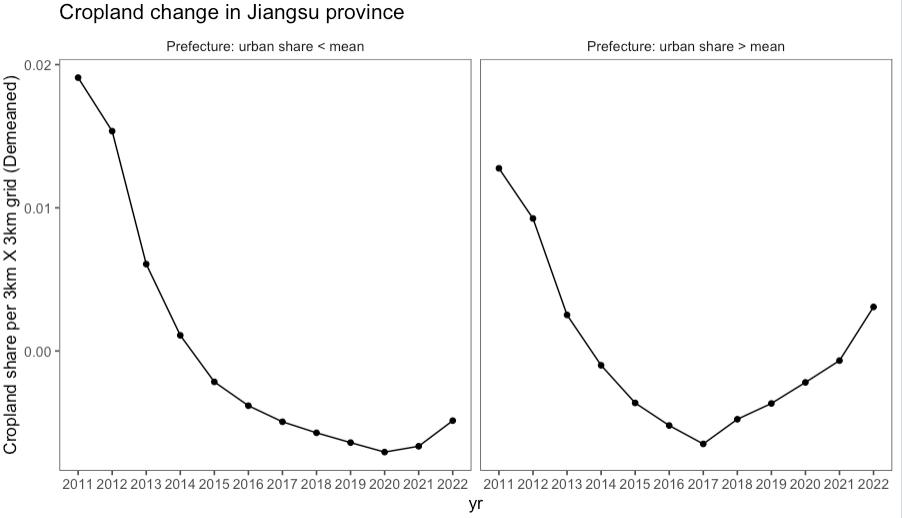
\includegraphics[width=0.8\textwidth]{cropland_jiangsu_urbanshare.png}
\end{figure}
\end{frame}

\begin{frame}{Descriptive statistics: high urban density v.s. low urban density}
\begin{figure}[H]
    \centering
    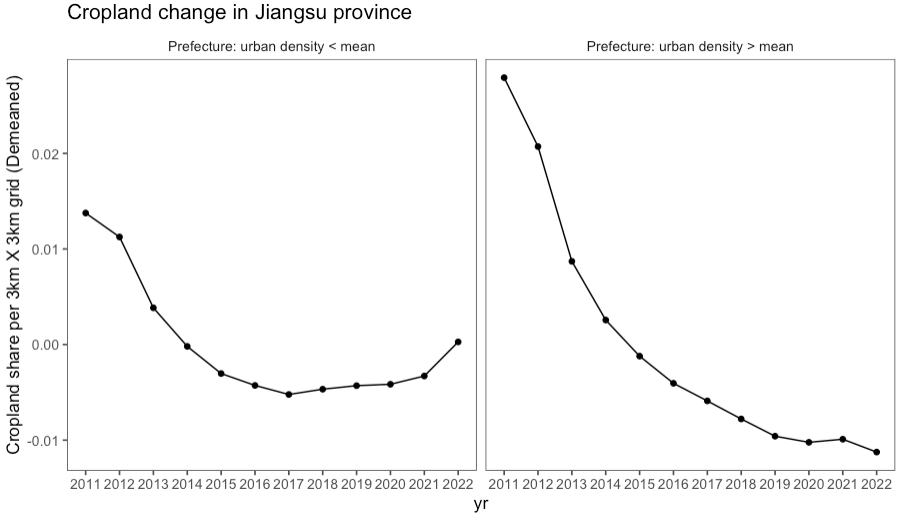
\includegraphics[width=0.8\textwidth]{cropland_jiangsu_urbandensity.png}
\end{figure}
\end{frame}

\begin{frame}{Descriptive statistics: cropland in Jiangsu province}
\begin{figure}[H]
    \centering
    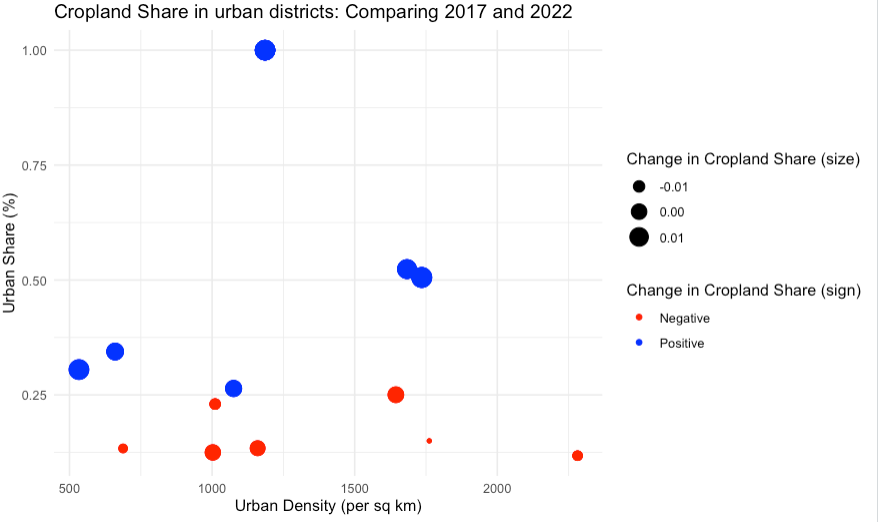
\includegraphics[width=0.8\textwidth]{cropshareurban_2217.png}
\end{figure}
\end{frame}

\begin{frame}{Descriptive statistics: cropland in Jiangsu province}
\begin{figure}[H]
    \centering
    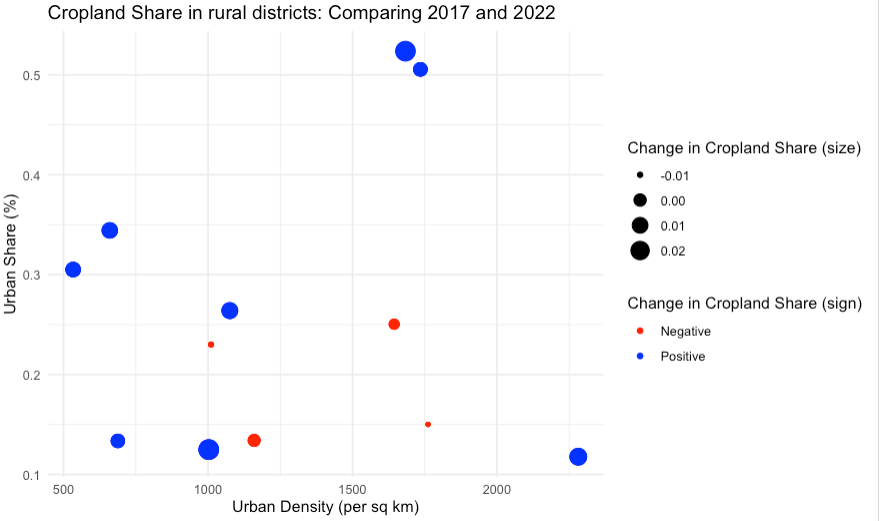
\includegraphics[width=0.8\textwidth]{cropsharerural_2217.png}
\end{figure}
\end{frame}